
\chapter{Baire Spaces and Dimension Theory}

In this chapter, we introduce a class of topological spaces called the \idx{Baire space}s. The defining condition for a Baire space is a bit complicated to state, but it is often useful in the applications, in both analysis and topology. Most of the spaces we have been studying are Baire spaces. For instance, a Hausdorff space is a Baire space if it is \idx{Compact Hausdorff space: is Baire space} compact, or even \idx{Locally compact Hausdorff space: Baire condition} locally compact. And a metrizable space \(X\) is a Baire space if It is topologically complete, that is, if there is a metric for \(X\) relative to which \(X\) is complete.

It follows that, since the space \(\mathcal{C}\left( {X,{\mathbb{R}}^{n}}\right)\) of all continuous functions from a space \(X\) to \({\mathbb{R}}^{n}\) is complete in the \idx{Uniform structure} uniform metric, it is a Baire space in the uniform topology. This fact has a number of interesting applications.

One application is the proof we give in \(\$ {49}\) of the existence of a continuous nowhere-differentiable real-valued function.

Another application arises in that branch of topology called \idx{Dimension, topological} dimension theory. In \(\$ {50}\) , we define a topological notion of dimension, due to Lebesgue. And we prove the classical theorem that every compact metrizable space of \idx{topological dimension} \(m\) can be imbedded in euclidean space \({\mathbb{R}}^{N}\) of dimension \(N = {2m} + 1\) . It follows that every compact \(m\) -manifold can be imbedded in \({\mathbb{R}}^{{2m} + 1}\) This generalizes the imbedding theorem proved in §36.

Throughout the chapter, we assume familiarity with complete metric spaces (§43). When we study dimension theory, we shall make use of §36, Imbeddings of Manifolds, as well as a bit of linear algebra.

\section*{§ 48 Baire Spaces}

The defining condition for a Baire space is probably as "unnatural looking" as any condition we have yet introduced in this book. But bear with us awhile.

In this section, we shall define Baure spaces and shall show that two important classes of spaces-the complete metric spaces and the compact Hausdorff spaces-are contained in the class of Baire spaces. Then we shall give some applications, which, even if they do not make the Baire condition seem any more natural, will at least show what a useful tool it can be. In fact, it turns out to be a very useful and fairly sophisticated tool in both analysis and topology.

\begin{definition} Recall that if \(A\) is a subset of a space \(X\) , the interior of \(A\) is defined as the union of all open sets of \(X\) that are contained in \(A\) . To say that \(A\) has \idx{empty interior} is to say then that \(A\) contains no open set of \(X\) other than the empty set. Equivalently, \(A\) has empty interior if every point of \(A\) is a limit point of the complement of \(A\) , that is, if the complement of \(A\) is dense in \(X\) .
\end{definition}

\begin{example} The set \(\mathbb{Q}\) of rationals has emply interior as a subset of \(\mathbb{R}\) , but the interval \(\left\lbrack  {0,1}\right\rbrack\) has nonempty interior The interval \(\left\lbrack  {0,1}\right\rbrack   \times  0\) has empty interior as a subset of the plane \({\mathbb{R}}^{2}\) , and so does the subset \(\mathbb{Q} \times  \mathbb{R}\) .
\end{example}

\begin{definition} A space \(X\) is said to be a Baire space if the following condition holds: Given any countable collection \(\left\{  {A}_{n}\right\}\) of closed sets of \(X\) each of which has empty interior in \(X\) , their union \(\bigcup {A}_{n}\) also has empty interior in \(X\) .
\end{definition}

\begin{example} The space \(\mathbb{Q}\) of rationals is not a Baire space. For each one-point set in \(\mathbb{Q}\) is closed and has empty interior in \(\mathbb{Q}\) , and \(\mathbb{Q}\) is the countable union of its one-point subsets.
\end{example}

The space \({\mathbb{Z}}_{ + }\) , on the other hand, does form a Baire space Every subset of \({\mathbb{Z}}_{ + }\) is open, so that there exist no subsets of \({\mathbb{Z}}_{ + }\) having empty interior, except for the empty set. Therefore, \({\mathbb{Z}}_{ + }\) satisfies the Baire condition vacuously.

More generally, every closed subspace of \(\mathbb{R}\) , being a complete metric space, is a Baire space. Somewhat surprising is the fact that the irrationals in \(\mathbb{R}\) also form a Baire space; see Exercise 6

The terminology originally used by R. Baire for this concept involved the word "category." A subset \(A\) of a space \(X\) was said to be of the \idx{First category set} first category in \(X\) if it was contained in the union of a countable collection of closed sets of \(X\) having empty interiors in \(X\) ; otherwise, it was said to be of the \idx{Second category set} second category in \(X\) . Using this terminology, we can say the following:

A space \(X\) is a Baire space if and only if every nonempty open set in \(X\) is ofthe second category

We shall not use the terms "first category" and "second category" in this book.

The preceding definition is the "closed set definition" of a Baire space. There is also a formulation involving open sets that is frequently useful. It is given in the following lemma.

\begin{lemma} \(X\) is a Baire space if and only if given any countable collection \(\left\{  {U}_{n}\right\}\) of open sets in \(X\) , each of which is dense in \(X\) , their intersection \(\cap  {U}_{n}\) is also dense in \(X\) .
\end{lemma}

\begin{proof}Recall that a set \(C\) is dense in \(X\) if \(\bar{C} = X\) . The theorem now follows at once from the two remarks:
(1) \(A\) is closed in \(X\) if and only if \(X - A\) is open in \(X\) .

(2) \(B\) has empty interior in \(X\) if and only if \(X - B\) is dense in \(X\) .

There are a number of theorems giving conditions under which a space is a Baire space. The most important is the following:
\end{proof}
\begin{theorem}[\idx{Baire category theorem}] If \(X\) is a compact Hausdorff space or a complete metric space, then \(X\) is a Baire space.
\end{theorem}

\begin{proof}Given a countable collection \(\left\{  {A}_{n}\right\}\) of closed set of \(X\) having empty interiors, we want to show that their union \(\bigcup {A}_{n}\) also has empty interior in \(X\) . So, given the nonempty open set \({U}_{0}\) of \(X\) , we must find a point \(x\) of \({U}_{0}\) that does not lie in any of the sets \({A}_{n}\) .
Consider the first set \({A}_{1}\) . By hypothesis, \({A}_{1}\) does not contain \({U}_{0}\) . Therefore, we may choose a point \(y\) of \({U}_{0}\) that is not in \({A}_{1}\) . Regularity of \(X\) , along with the fact that \({A}_{1}\) is closed, enables us to choose a neighborhood \({U}_{1}\) of \(y\) such that

\[
{\bar{U}}_{1} \cap  {A}_{1} = \varnothing
\]

\[
{\bar{U}}_{1} \subset  {U}_{0}\text{ . }
\]

If \(X\) is metric, we also choose \({U}_{1}\) small enough that its diameter is less than1.

In general, given the nonempty open set \({U}_{n - 1}\) , we choose a point of \({U}_{n - 1}\) that is not in the closed set \({A}_{n}\) , and then we choose \({U}_{n}\) to be a neighborhood of this point such that

\[
{\bar{U}}_{n} \cap  {A}_{n} = \varnothing
\]

\[
{\bar{U}}_{n} \subset  {U}_{n - 1},
\]

\[
\text{ diam }{U}_{n} < 1/n\text{ in the metric case. }
\]

We assert that the intersection \(\cap  {\bar{U}}_{n}\) is nonempty. From this fact, our theorem will follow. For if \(x\) is a point of \(\bigcap {\bar{U}}_{n}\) , then \(x\) is in \({U}_{0}\) because \({\bar{U}}_{1} \subset  {U}_{0}\) . And for each \(n\) , the point \(x\) is not in \({A}_{n}\) because \({\bar{U}}_{n}\) is disjoint from \({A}_{n}\) .

The proof that \(\cap  {\widetilde{U}}_{n}\) is nonempty splits into two parts, depending on whether \(X\) is compact Hausdorff or complete metric. If \(X\) is compact Hausdorff, we consider the nested sequence \({\bar{U}}_{1} \supset  {\bar{U}}_{2} \supset  \cdots\) of nonempty subsets of \(X\) . The collection \(\left\{  {\bar{U}}_{n}\right\}\) has the finite intersection property; since \(X\) is compact, the intersection \(\cap  {U}_{n}\) must be nonempty.

If \(X\) is complete metric, we apply the following lemma.
\end{proof}
\begin{lemma} Let \({C}_{1} \supset  {C}_{2} \supset   \cdot   \cdot\) be a nested sequence of nonempty closed sets in the complete metric space \(X\) . If \(\operatorname{diam}{C}_{n} \rightarrow  0\) , then \(\cap  {C}_{n} \neq  \varnothing\) .
\end{lemma}

\begin{proof}We gave this as an exercise in \(§{43}\) . Here is a proof: Choose \({x}_{n} \in  {C}_{n}\) for each \(n\) . Because \({x}_{n},{x}_{m} \in  {C}_{N}\) for \(n,m \geq  N\) , and because \(\operatorname{diam}{C}_{N}\) can be made less than any given \(\epsilon\) by choosing \(N\) large enough, the sequence \(\left( {x}_{n}\right)\) is a Cauchy sequence. Suppose that it converges to \(x\) . Then for given \(k\) , the subsequence \({x}_{k},{x}_{k + 1},\ldots\) also converges to \(x\) . Thus \(x\) necessarily belongs to \({\widetilde{C}}_{k} = {C}_{k}\) . Then \(x \in  \bigcap {C}_{k}\) , as desired.
Here is one application of the theory of Baire spaces; we shall give further applications in the sections that follow. This application is perhaps more amusing than profound. It concerns a question that a student might ask concerning convergent sequences of continuous functions.

Let \({f}_{n} : \left\lbrack  {0,1}\right\rbrack   \rightarrow  \mathbb{R}\) be a sequence of continuous functions such that \({f}_{n}\left( x\right)  \rightarrow\)  \(f\left( x\right)\) for each \(x \in  \left\lbrack  {0,1}\right\rbrack\) . There are examples that show the limit function \(f\) need not be continuous. But one might wonder just how discontinuous \(f\) can be Could it be discontinuous everywhere, for instance? The answer is "no." We shall show that \(f\) must be continuous at infinitely many \idx{End points of arc} points of \(\left\lbrack  {0,1}\right\rbrack\) . In fact, the set of points at which \(f\) is continuous is dense in \(\left\lbrack  {0,1}\right\rbrack\) !

To prove this result, we need the following lemma:

*Lemma 48.4. Any open subspace \(Y\) of a Baire space \(X\) is itself a Baire space.

Proof. Let \({A}_{n}\) be a countable collection of closed sets of \(Y\) that have empty interiors in \(Y\) . We show that \(\bigcup {A}_{n}\) has empty interior in \(Y\) .

Let \({\bar{A}}_{n}\) be the closure of \({A}_{n}\) in \(X\) ; then \({\bar{A}}_{n} \cap  Y = {A}_{n}\) . The set \({\bar{A}}_{n}\) has empty interior in \(X\) . For if \(U\) is a nonempty open set of \(X\) contained in \({\bar{A}}_{n}\) , then \(U\) must intersect \({A}_{n}\) . Then \(U \cap  Y\) is a nonempty open set of \(Y\) contained in \({A}_{n}\) , contrary to hypothesis

If the union of the sets \({A}_{n}\) contains the nonempty open set \(W\) of \(Y\) , then the union of the sets \({A}_{n}\) also contains the set \(W\) , which is open in \(X\) because \(Y\) is open in \(X\) . But each set \({\bar{A}}_{n}\) has empty interior in \(X\) , contradicting the fact that \(X\) is a Baire space.

*Theorem 48.5. Let \(X\) be a space; let(Y, d)be a metric space. Let \({f}_{n} : X \rightarrow  Y\) be a sequence of continuous functions such that \({f}_{n}\left( x\right)  \rightarrow  f\left( x\right)\) for all \(x \in  X\) , where \(f : X \rightarrow  Y\) . If \(X\) is a Baire space, the set of points at which \(f\) is continuous is dense in \(X\) .

Proof. Given a positive integer \(N\) and given \(\epsilon  > 0\) , define

\[
{A}_{N}\left( \epsilon \right)  = \left\lbrack  {x \mid  d\left( {{f}_{n}\left( x\right) ,{f}_{m}\left( x\right) }\right)  \leq  \epsilon }\right. \text{ for all }\left. {n,m \geq  N}\right\}  \text{ . }
\]

Note that \({A}_{N}\left( \epsilon \right)\) is closed in \(X\) . For the set of those \(x\) for which \(d\left( {{f}_{n}\left( x\right) ,{f}_{m}\left( x\right) }\right)  \leq  \epsilon\) is closed in \(X\) , by continuity of \({f}_{n}\) and \({f}_{m}\) , and \({A}_{N}\left( \epsilon \right)\) is the intersection of these sets for all \(n,m \geq  N\) .

For fixed \(\epsilon\) , consider the sets \({A}_{1}\left( \epsilon \right)  \subset  {A}_{2}\left( \epsilon \right)  \subset  \cdots\) . The union of these sets is all of \(X\) . For, given \({x}_{0} \in  X\) , the fact that \({f}_{n}\left( {x}_{0}\right)  \rightarrow  f\left( {x}_{0}\right)\) implies that the sequence \({f}_{n}\left( {x}_{0}\right)\) is a Cauchy sequence; hence \({x}_{0} \in  {A}_{N}\left( \epsilon \right)\) for some \(N\) .

Now let

\[
U\left( \epsilon \right)  = \mathop{\bigcup }\limits_{{N \in  {\mathbf{Z}}_{ + }}}\operatorname{Int}{A}_{N}\left( \epsilon \right)
\]

We shall prove two things:

(1) \(U\left( \epsilon \right)\) is open and dense in \(X\) .

(2) The function \(f\) is continuous at each point of the set

\[
C = U\left( 1\right)  \cap  U\left( {1/2}\right)  \cap  U\left( {1/3}\right)  \cap  \cdots .
\]

Our theorem then follows from the fact that \(X\) is a Baire space.

To show that \(U\left( \epsilon \right)\) is dense in \(X\) , it suffices to show that for any nonempty open set \(V\) of \(X\) , there is an \(N\) such that the set \(V \cap  \operatorname{Int}{A}_{N}\left( \epsilon \right)\) is nonempty. For this purpose, we note first that for each \(N\) , the set \(V \cap  {A}_{N}\left( \epsilon \right)\) is closed in \(V\) . Because \(V\) is a Baire space by the preceding lemma, at least one of these sets, say \(V \cap  {A}_{M}\left( \epsilon \right)\) , must contain a nonempty open set \(W\) of \(V\) Because \(V\) is open in \(X\) , the set \(W\) is open in \(X\) ; therefore, it is contained in Int \({A}_{M}\left( \epsilon \right)\) .

Now we show that if \({x}_{0} \in  C\) , then \(f\) is continuous at \({x}_{0}\) . Given \(\epsilon  > 0\) , we shall find a neighborhood \(W\) of \({x}_{0}\) such that \(d\left( {f\left( x\right) ,f\left( {x}_{0}\right) }\right)  < \epsilon\) for \(x \in  W\) .

First, choose \(k\) so that \(1/k < \epsilon /3\) . Since \({x}_{0} \in  C\) , we have \({x}_{0} \in  U\left( {1/k}\right)\) ; therefore, there is an \(N\) such that \({x}_{0} \in  \operatorname{Int}{A}_{N}\left( {1/k}\right)\) . Finally, continuity of the function \({f}_{N}\) enables us to choose a neighborhood \(W\) of \({x}_{0}\) , contained in \({A}_{N}\left( {1/k}\right)\) , such that

(*)
\[
d\left( {{f}_{N}\left( x\right) ,{f}_{N}\left( {x}_{0}\right) }\right)  < \epsilon /3\;\text{ for }x \in  W.
\]

The fact that \(W \subset  {A}_{N}\left( {1/k}\right)\) implies that

\[
d\left( {{f}_{n}\left( x\right) ,{f}_{N}\left( x\right) }\right)  \leq  1/k\;\text{ for }n \geq  N\text{ and }x \in  W.
\]

Letting \(n \rightarrow  \infty\) , we obtain the inequality

\[
\left( {* * }\right)
\]

\[
d\left( {f\left( x\right) ,{f}_{N}\left( x\right) }\right)  \leq  1/k < \epsilon /3\;\text{ for }x \in  W.
\]

In particular, since \({x}_{0} \in  W\) , we have

\[
\left( {* *  * }\right)
\]

\[
d\left( {f\left( {x}_{0}\right) ,{f}_{N}\left( {x}_{0}\right) }\right)  < \epsilon /3.
\]

Applying the triangle inequality to \(\left( *\right) ,\left( {* * }\right)\) , and \(\left( {* *  * }\right)\) gives us our desired result.
\end{proof}
\section*{Exercises}

1. Let \(X\) equal the countable union \(\cup  {B}_{n}\) . Show that if \(X\) is a nonempty Baire space, at least one of the sets \({\bar{B}}_{n}\) has a nonempty interior.

2. The Baire category theorem implies that \(\mathbb{R}\) cannot be written as a countable union of closed subsets having empty interiors. Show this fails if the sets are not required to be closed

3. Show that every locally compact Hausdorff space is a Baire space.

4. Show that if every point \(x\) of \(X\) has a neighborhood that is a Barre space, then \(X\) is a Baure space. [Hint: Use the open set formulation of the Baure condition.\}

5. Show that if \(Y\) is a \({G}_{\delta }\) set in \(X\) , and if \(X\) is compact Hausdorff or complete metric, then \(Y\) is a Baire space in the subspace topology. [Hint: Suppose that \(Y = \bigcap {W}_{n}\) , where \({W}_{n}\) is open in \(X\) , and that \({B}_{n}\) is closed in \(Y\) and has empty interior in \(Y\) . Given \({U}_{0}\) open in \(X\) with \({U}_{0} \cap  Y \neq  \varnothing\) , find a sequence of open sets \({U}_{n}\) of \(X\) with \({U}_{n} \cap  Y\) nonempty, such that

\[
{\bar{U}}_{n} \subset  {U}_{n - 1},
\]

\[
{\bar{U}}_{n} \cap  {\bar{B}}_{n} = \varnothing
\]

\[
\operatorname{diam}{U}_{n} < 1/n\;\text{ in the metric case, }
\]

\[
\left. {{\bar{U}}_{n} \subset  {W}_{n}}\right\}
\]

6. Show that the irrationals are a Baire space.

7. Prove the following:

\begin{theorem} If \(D\) is a countable dense subset of \(\mathbb{R}\) , there is no function \(f : \mathbb{R} \rightarrow  \mathbb{R}\) that is continuous precisely at the points of \(D\)
\end{theorem}

Proof.

(a) Show that if \(f : \mathbb{R} \rightarrow  \mathbb{R}\) , then the set \(C\) of points at which \(f\) is continuous is a \({G}_{\delta }\) set in \(\mathbb{R}\) . [Hint: Let \({U}_{n}\) be the union of all open sets \(U\) of \(\mathbb{R}\) such that \(\operatorname{diam}f\left( U\right)  < 1/n\) . Show that \(C = \bigcap {U}_{n}\) .\}

(b) Show that \(D\) is not a \({G}_{\delta }\) set in \(\mathbb{R}\) . [Hint: Suppose \(D = \bigcap {W}_{n}\) , where \({W}_{n}\) is open in \(\mathbb{R}\) . For \(d \in  D\) , set \({V}_{d} = \mathbb{R} - \lbrack d\}\) . Show \({W}_{n}\) and \({V}_{d}\) are dense in \(\mathbb{R}\) .

8. If \({f}_{n}\) is a sequence of continuous functions \({f}_{n} : \mathbb{R} \rightarrow  \mathbb{R}\) such that \({f}_{n}\left( x\right)  \rightarrow  f\left( x\right)\) for each \(x \in  \mathbb{R}\) , show that \(f\) is continuous at uncountably many points of \(\mathbb{R}\) .

9. Let \(g : {\mathbb{Z}}_{ + } \rightarrow  \mathbb{Q}\) be a bijective function; let \({x}_{n} = g\left( n\right)\) . Define \(f : \mathbb{R} \rightarrow  \mathbb{R}\) as follows:

\[
f\left( {x}_{n}\right)  = 1/n\;\text{ for }{x}_{n} \in  \mathbb{Q},
\]

\[
f\left( x\right)  = 0\;\text{ for }x \notin  \mathbb{Q}
\]

Show that \(f\) is continuous at each irrational and discontinuous at each rational. Can you find a sequence of continuous functions \({f}_{n}\) coverging to \(f\) ?

10. Prove the following:

\begin{theorem}[\idx{Uniform boundedness principle}] Let \(X\) be a complete metric space, and let \(\mathcal{F}\) be a subset of \(\mathcal{C}\left( {X,\mathbb{R}}\right)\) such that for each \(a \in  X\) , the set

\[
{\mathcal{F}}_{a} = \{ f\left( a\right)  \mid  f \in  \mathcal{F}\}
\]

is bounded. Then there is a nonempty open set \(U\) of \(X\) on which the functions in \(\mathcal{F}\) are uniformly bounded, that is, there is a number \(M\) such that \(\left| {f\left( x\right) }\right|  \leq  M\) for all \(x \in  U\) and all \(f \in  \mathcal{F}\) . [Hint: Let \({A}_{N} = \{ x;\left| {f\left( x\right) }\right|  \leq  N\) for all \(f \in  \mathcal{F}\}\) .]
\end{theorem}

11. Determine whether or not \({\mathbb{R}}_{\ell }\) is a Baire space

12. Show that \({\mathbb{R}}^{J}\) is a Baire space in the box, product, and uniform topologies.

*13. Let \(X\) be a topological space; let \(Y\) be a complete metric space. Show that \(\mathcal{C}\left( {X,Y}\right)\) is a Baire space in the fine topology (see Exercise 11 of §46). [Hint: Given basis elements \(B\left( {{f}_{i},{\delta }_{i}}\right)\) such that \({\delta }_{1} \leq  1\) and \({\delta }_{i + 1} \leq  {\delta }_{i}/3\) and \({f}_{i + 1} \in\)  \(B\left( {{f}_{i},{\delta }_{i}/3}\right)\) , show that

\[
\bigcap B\left( {{f}_{i},{\delta }_{i}}\right)  \neq  \varnothing \text{ .] }
\]

\section*{*§ 49 A Nowhere-Differentiable Function}

We prove the following result from analysis:

\begin{theorem} Let \(h : \left\lbrack  {0,1}\right\rbrack   \rightarrow  \mathbb{R}\) be a continuous function. Given \(\epsilon  > 0\) , there is a function \(g : \left\lbrack  {0,1}\right\rbrack   \rightarrow  \mathbb{R}\) with \(\left| {h\left( x\right)  - g\left( x\right) }\right|  < \epsilon\) for all \(x\) , such that \(g\) is continuous and nowhere differentiable.
\end{theorem}

\begin{proof}Let \(I = \left\lbrack  {0,1}\right\rbrack\) . Consider the space \(\mathcal{C} = \mathcal{C}\left( {I,\mathbb{R}}\right)\) of continuous maps from \(I\) to \(\mathbb{R}\) , in the metric
\[
\rho \left( {f,g}\right)  = \max \{ \left| {f\left( x\right)  - g\left( x\right) }\right| \} .
\]

This space is a complete metric space and, therefore, is a Bare space. We shall define, for each \(n\) , a certain subset \({U}_{n}\) of \(\mathcal{C}\) that is open in \(\mathcal{C}\) and dense in \(\mathcal{C}\) , and has the property that the functions belonging to the intersection

\[
\mathop{\bigcap }\limits_{{n \in  {\mathbf{Z}}_{ + }}}{U}_{n}
\]

are nowhere differentiable. Because \(\mathcal{C}\) is a Baire space, this intersection is dense in \(\mathcal{C}\) , by Lemma 48.1. Therefore, given \(h\) and \(\epsilon\) , this intersection must contain a function \(g\) such that \(\rho \left( {h,g}\right)  < \epsilon\) . The theorem follows.

The tricky part is to define the set \({U}_{n}\) properly. We first take a function \(f\) and consider its difference quotients. Given \(x \in  I\) and given \(0 < h \leq  \frac{1}{2}\) , consider the expressions

\[
\left| \frac{f\left( {x + h}\right)  - f\left( x\right) }{h}\right| \;\text{ and }\;\left| \frac{f\left( {x - h}\right)  - f\left( x\right) }{-h}\right| .
\]

Since \(h \leq  \frac{1}{2}\) , at least one of the numbers \(x + h\) and \(x - h\) belongs to \(I\) , so that at least one of these expressions is defined. Let \({\Delta f}\left( {x,h}\right)\) denote the larger of the two if both are defined; otherwise, let it denote the one that is defined. If the derivative \({f}^{\prime }\left( x\right)\) of \(f\) at \(x\) exists, it equals the limit of these difference quotients, so that

\[
\left| {{f}^{\prime }\left( x\right) }\right|  = \mathop{\lim }\limits_{{h \rightarrow  0}}{\Delta f}\left( {x,h}\right) .
\]

We seek to find a continuous function for which this limit does not exist. To be specific, we shall construct \(f\) so that given \(x\) , there is a sequence of numbers \({h}_{n}\) converging to 0 for which the numbers \({\Delta f}\left( {x,{h}_{n}}\right)\) become arbitrarily large.

This gives us the idea for defining the set \({U}_{n}\) . Given any positive number \(h \leq  1/2\) , let

\[
{\Delta }_{h}f = \inf \{ {\Delta f}\left( {x,h}\right)  \mid  x \in  I\}
\]

Then for \(n \geq  2\) , we define \({U}_{n}\) by declaring that a function \(f\) belongs to \({U}_{n}\) if and only if for some positive number \(h \leq  1/n\) , we have \({\Delta }_{h}f > n\) .

\begin{example} Let \(\alpha  > 0\) be given. The function \(f.\left\lbrack  {0,1}\right\rbrack   \rightarrow  \mathbb{R}\) given by the equation \(f\left( x\right)  = {4\alpha x}\left( {1 - x}\right)\) , whose \idx{Utilities graph} graph is a parabola, satisfies the condition \({\Delta f}\left( {x,h}\right)  \geq  \alpha\) for \(h = 1/4\) and all \(x\) , as you can check Geometrically speaking, what this says is that for each \(x\) , at least one of the indicated secant lines of the parabola in Figure 49.1 has slope of absolute value at least \(\alpha\) . Hence if \(\alpha  > 4\) , the function \(f\) belongs to \({U}_{4}\) The function \(g\) pictured in Figure 49.1 satisfies the condition \({\Delta g}\left( {x,h}\right)  \geq  \alpha\) for any \(h \leq  1/4\) ; hence \(g\) belongs to \({U}_{n}\) provided \(\alpha  > n\) . The function \(k\) satisfies the condition \(k\left( {x,h}\right)  \geq  \alpha\) for any \(h \leq  1/8\) ; hence \(k\) belongs to \({U}_{n}\) if \(\alpha  > n\) .

\begin{center}
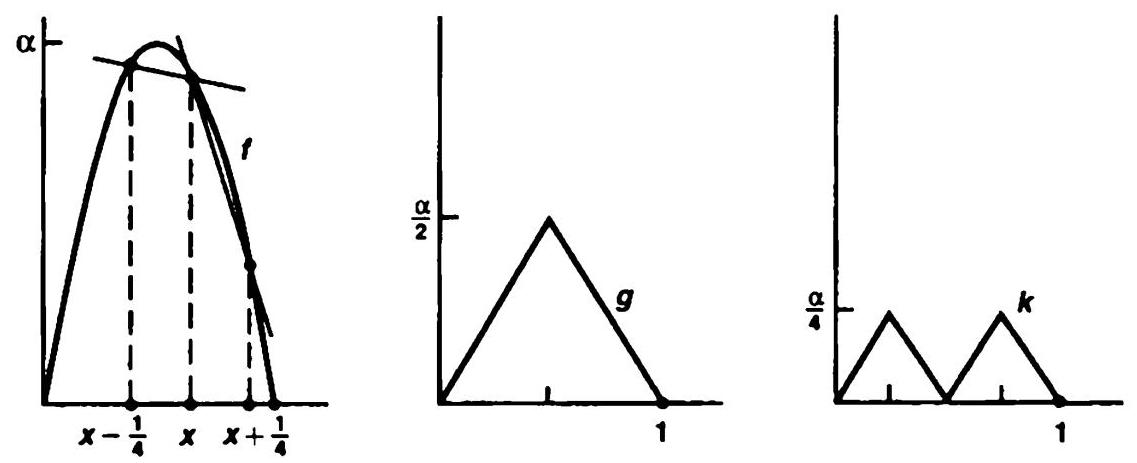
\includegraphics[width=1.0\textwidth]{images/49.1.jpg}
\end{center}
\hspace*{3em} 

Figure 49.1
\end{example}

Now we prove the following facts about the set \({U}_{n}\) :

(1) \(\bigcap {U}_{n}\) consists of \idx{nowhere-differentiable function}s. Let \(f \in  \bigcap {U}_{n}\) . We shall prove that given \(x\) in \(\left\lbrack  {0,1}\right\rbrack\) , the limit

\[
\lim {\Delta f}\left( {x,h}\right)
\]

does not exist: Given \(n\) , the fact that \(f\) belongs to \({U}_{n}\) means that we can find a number \({h}_{n}\) with \(0 < {h}_{n} \leq  1/n\) such that

\[
{\Delta f}\left( {x,{h}_{n}}\right)  > n\text{ . }
\]

Then the sequence \(\left( {h}_{n}\right)\) converges to zero, but the sequence \(\left( {{\Delta f}\left( {x,{h}_{n}}\right) }\right)\) does not converge. As a result, \(f\) is not differentiable at \(x\) .

(2) \({U}_{n}\) is open in \(\mathcal{C}\) . Suppose that \(f \in  {U}_{n}\) ; we find a \(\delta\) -neighborhood of \(f\) that is contained in \({U}_{n}\) . Because \(f \in  {U}_{n}\) , there is a number \(h\) with \(0 < h \leq  1/n\) such that \({\Delta }_{h}f > n\) . Set \(M = {\Delta }_{h}f\) , and let

\[
\delta  = h\left( {M - n}\right) /4
\]

We assert that if \(g\) is a function with \(\rho \left( {f,g}\right)  < \delta\) , then

\[
{\Delta g}\left( {x,h}\right)  \geq  \frac{1}{2}\left( {M + n}\right)  > n
\]

for all \(x \in  I\) , so that \(g \in  {U}_{n}\) .

To prove the assertion, let us first assume that \({\Delta f}\left( {x,h}\right)\) is equal to the quotient \(\left| {f\left( {x + h}\right)  - f\left( x\right) }\right| /h\) . We compute

\[
\left| {\frac{f\left( {x + h}\right)  - f\left( x\right) }{h} - \frac{g\left( {x + h}\right)  - g\left( x\right) }{h}}\right|  =
\]

\[
\left( {1/h}\right) \left| {\left\lbrack  {f\left( {x + h}\right)  - g\left( {x + h}\right) }\right\rbrack   - \left\lbrack  {f\left( x\right)  - g\left( x\right) }\right\rbrack  }\right|  \leq  {2\delta }/h = \left( {M - n}\right) /2.
\]

If the first difference quotient is at least \(M\) in absolute value, then the second is in absolute value at least

\[
M - \frac{1}{2}\left( {M - n}\right)  = \frac{1}{2}\left( {M + n}\right) .
\]

A similar remark applies if \({\Delta f}\left( {x,h}\right)\) equals the other difference quotient.

(3) \({U}_{n}\) is dense in \(\mathcal{C}\) . We must show that given \(f\) in \(\mathcal{C}\) , given \(\epsilon  > 0\) , and given \(n\) , we can find an element \(g\) of \({U}_{n}\) within \(\epsilon\) of \(f\) .

Choose \(\alpha  > n\) . We shall construct \(g\) as a "\idx{Piecewise linear function} piecewise-linear" function, that is, a function whose graph is a broken line segment; each line segment in the graph of \(g\) will have slope at least \(\alpha\) in absolute value. It follows at once that such a function \(g\) belongs to \({U}_{n}\) . For let

\[
0 = {x}_{0} < {x}_{1} < {x}_{2} < \cdots  < {x}_{k} = 1
\]

be a partition of the interval \(\left\lbrack  {0,1}\right\rbrack\) such that the restriction of \(g\) to each subinterval \({I}_{i} = \left\lbrack  {{x}_{i - 1},{x}_{i}}\right\rbrack\) is a linear function. Then choose \(h\) so that \(h \leq  1/n\) and

\[
h \leq  \frac{1}{2}\min \left\{  {\left| {{x}_{i} - {x}_{i - 1}}\right| ;i = 1,\ldots ,k}\right\}  .
\]

If \(x\) is in \(\left\lbrack  {0,1}\right\rbrack\) , then \(x\) belongs to some subinterval \({I}_{i}\) . If \(x\) belongs to the first half of the subinterval \({I}_{i}\) , then \(x + h\) belongs to \({I}_{i}\) and \(\left( {g\left( {x + h}\right)  - g\left( x\right) }\right) /h\) equals the slope of the linear function \(g \mid  {I}_{i}\) Similarly, if \(x\) belongs to the second half of \({I}_{i}\) , then \(x - h\) belongs to \({I}_{i}\) and \(\left( {g\left( {x - h}\right)  - g\left( x\right) }\right) /\left( {-h}\right)\) equals the slope of \(g \mid  {I}_{i}\) . In either case, \({\Delta g}\left( {x,h}\right)  \geq  \alpha\) , so \(g \in  {U}_{n}\) , as desired.

Now given \(f,\epsilon\) , and \(\alpha\) , we must show how to construct the desired piecewise-linear function \(g\) . First, we use uniform continuity of \(f\) to choose a partition of the interval

\[
0 = {t}_{0} < {t}_{1} < \cdots  < {t}_{m} = 1
\]

having the property that \(f\) varies by at most \(\epsilon /4\) on each subinterval \(\left\lbrack  {{t}_{i - 1},{t}_{i}}\right\rbrack\) of this partition. For each \(i = 1,\ldots ,m\) , choose a point \({a}_{i} \in  \left( {{t}_{i - 1},{t}_{i}}\right)\) . We then define a piecewise-linear function \({g}_{1}\) by the equations

\[
{g}_{1}\left( x\right)  = \left\{  \begin{array}{ll} f\left( {t}_{i - 1}\right) & \text{ for }x \in  \left\lbrack  {{t}_{i - 1},{a}_{i}}\right\rbrack  , \\  f\left( {t}_{i - 1}\right)  + {m}_{i}\left( {x - {a}_{i}}\right) & \text{ for }x \in  \left\lbrack  {{a}_{i},{t}_{l}}\right\rbrack  , \end{array}\right.
\]

where \({m}_{i} = \left( {f\left( {t}_{i}\right)  - f\left( {t}_{i - 1}\right) }\right) /\left( {{t}_{i} - {a}_{i}}\right)\) . The graphs of \(f\) and \({g}_{1}\) are pictured in Figure 49.2.

\begin{center}
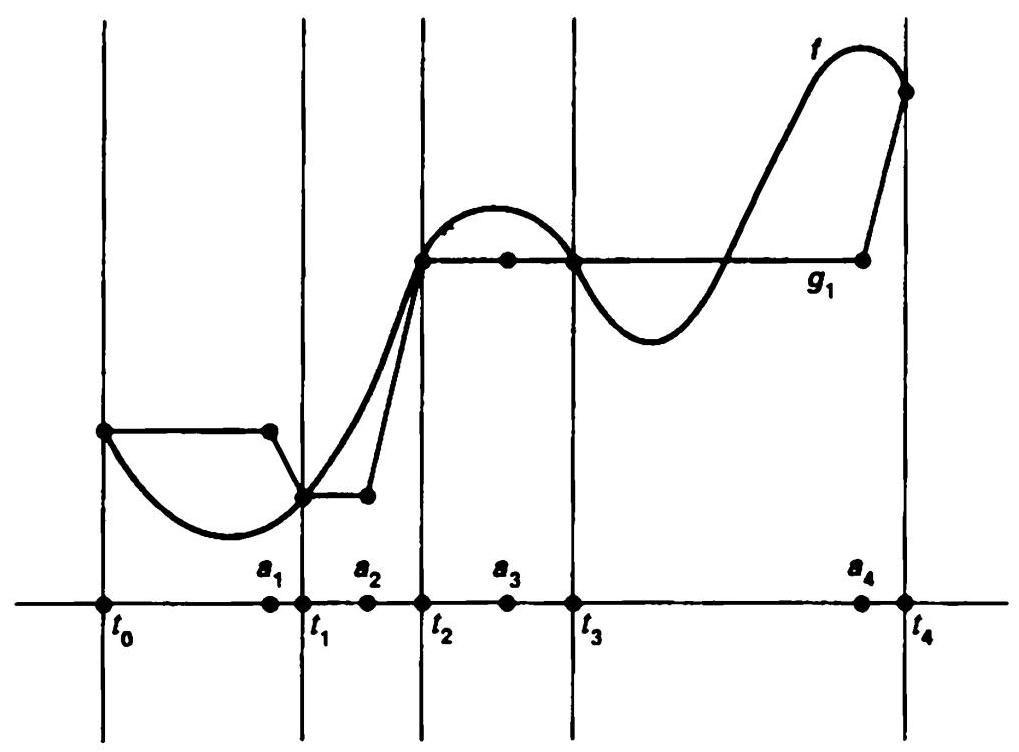
\includegraphics[width=0.9\textwidth]{images/49.2.jpg}
\end{center}
\hspace*{3em} 

Figure 49.2

We have some freedom of choice in choosing the point \({a}_{i}\) . If \(f\left( {t}_{i}\right)  \neq  f\left( {t}_{i - 1}\right)\) , we require \({a}_{i}\) to be close enough to \({t}_{i}\) that

\[
{t}_{i} - {a}_{i} < \frac{\left| f\left( {t}_{i}\right)  - f\left( {t}_{i - 1}\right) \right| }{\alpha }
\]

Then the graph of \({g}_{1}\) will consist entirely of line segments of slope zero and line segments of slope at least \(\alpha\) in absolute value.

Furthermore, we assert that \(\rho \left( {{g}_{1},f}\right)  \leq  \epsilon /2\) . On the interval \({I}_{i}\) , both \({g}_{1}\left( x\right)\) and \(f\left( x\right)\) vary by at most \(\epsilon /4\) from \(f\left( {t}_{i - 1}\right)\) ; therefore, they are within \(\epsilon /2\) of each other. Then \(\rho \left( {{g}_{1},f}\right)  = \max \left\lbrack  \left| {{g}_{1}\left( x\right)  - f\left( x\right) }\right| \right\}   \leq  \epsilon /2\) .

\begin{center}
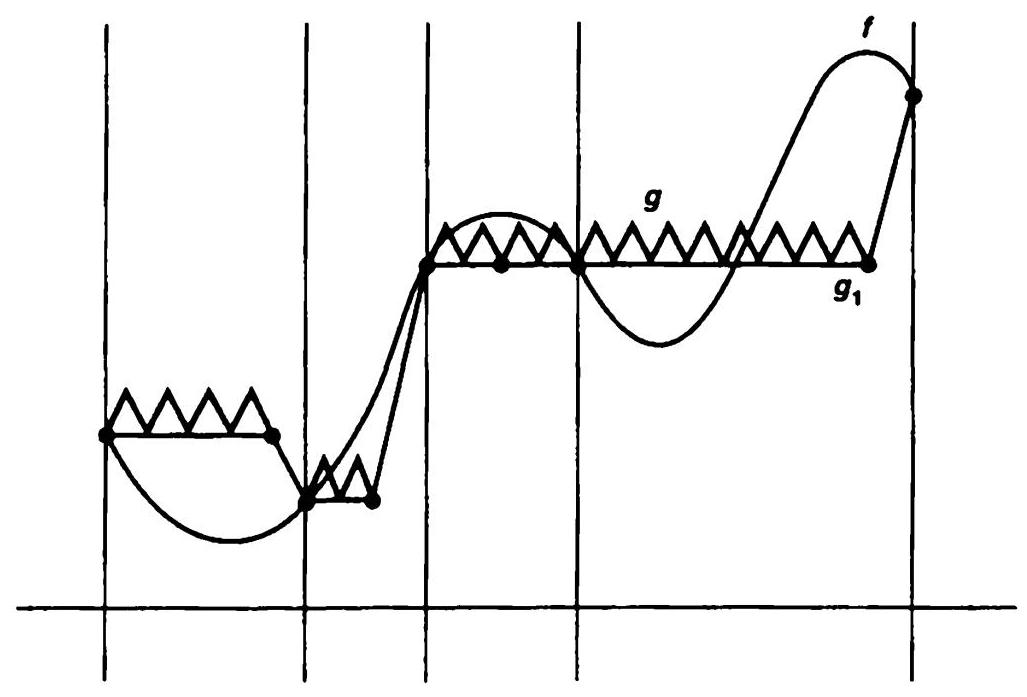
\includegraphics[width=0.9\textwidth]{images/49.3.jpg}
\end{center}
\hspace*{3em} 

Figure 49.3

The function \({g}_{1}\) is not yet the function we want. We now define a function \(g\) by replacing each horizontal line segment in the graph of \({g}_{1}\) by a "sawtooth" graph that lies within \(\epsilon /2\) of the graph of \({g}_{1}\) and has the property that each edge of the sawtooth has slope at least \(\alpha\) in absolute value. We leave this part of the construction to you. The result is the desired piecewise-linear function \(g\) . See Figure 49.3.

You may find this proof frustrating, in that it seems so abstract and nonconstructive. Implicit in the proof, however, is a procedure for constructing a specific sequence \({f}_{n}\) of piecewise-linear functions that converges uniformly to the nowhere-differentiable function \(f\) . And defining the function \(f\) in this way is just as constructive as the usual definition of the sine function, for instance, as the limit of an infinite senes.
\end{proof}
\section*{Exercises}

1. Check the stated properties of the functions \(f,g\) , and \(k\) of Example 1.

2. Given \(n\) and \(\epsilon\) , define a continuous function \(f : I \rightarrow  \mathbb{R}\) such that \(f \in  {U}_{n}\) and \(\left| {f\left( x\right) }\right|  \leq  \epsilon\) for all \(x\) .

\section*{§ 50 Introduction to Dimension Theory}

We showed in \(§{36}\) that if \(X\) is a compact manifold, then \(X\) can be imbedded in \({\mathbb{R}}^{N}\) for some positive integer \(N\) . In this section, we generalize this theorem to arbitrary compact metrizable spaces

We shall define, for an arbitrary topological space \(X\) , a notion of topological dimension. It is the "\idx{covering dimension}" originally defined by Lebesgue We shall prove that each compact subset of \({\mathbb{R}}^{m}\) has topological dimension at most \(m\) . We shall also prove that the topological dimension of any compact \(m\) -manifold is at most \(m\) . (It is, in fact, precisely \(m\) , but this we shall not prove.)

The major theorem of this section is the theorem, due to K. Menger and G. Nöbel-ing, that any compact metrizable space of topological dimension \(m\) can be imbedded in \({\mathbb{R}}^{N}\) for \(N = {2m} + 1\) . The proof is an application of the Baire theorem. It follows that every compact \(m\) -manifold can be imbedded in \({\mathbb{R}}^{{2m} + 1}\) . It follows also that a compact metrizable space can be imbedded in \({\mathbb{R}}^{N}\) for some \(N\) if and only if it has finite topological dimension.

Much of what we shall do holds without requiring the space in question to be compact. But we shall restrict ourselves to that case whenever it is convenient to do so. Generalizations to the noncompact case are given in the exercises.

\begin{definition} A collection \(\mathcal{A}\) of subsets of the space \(X\) is said to have \idx{Order of a covering} order \(m + 1\) if some point of \(X\) lies in \(m + 1\) elements of \(\mathcal{A}\) , and no point of \(X\) lies in more than \(m + 1\) elements of \(\mathcal{A}\) .
\end{definition}

Now we define what we mean by the topological dimension of a space \(X\) Recall that given a collection \(\mathcal{A}\) of subsets of \(X\) , a collection \(\mathcal{B}\) is said to refine \(\mathcal{A}\) , or to be a refinement of \(\mathcal{A}\) , if for each element \(B\) of \(\mathcal{B}\) there is an element \(A\) of \(\mathcal{A}\) such that \(B \subset  A\) .

\begin{definition} A space \(X\) is said to be \idx{finite dimensional} if there is some integer \(m\) such that for every open covering \(\mathcal{A}\) of \(X\) , there is an open covering \(\mathcal{B}\) of \(X\) that refines \(\mathcal{A}\) and has order at most \(m + 1\) . The topological dimension of \(X\) is defined to be the smallest value of \(m\) for which this statement holds; we denote it by \(\dim X\) .
\end{definition}

\begin{example} Any compact subspace \(X\) of \(\mathbb{R}\) has topological dimension at most 1. We begin by defining an open covering of \(\mathbb{R}\) of order 2 Let \({\mathcal{A}}_{1}\) denote the collection of all open intervals of the form \(\left( {n,n + 1}\right)\) in \(\mathbb{R}\) , where \(n\) is an integer. Let \({\mathcal{A}}_{0}\) denote the collection of all open intervals of the form \(\left( {n - 1/2,n + 1/2}\right)\) , for \(n\) an integer. Then \(\mathcal{A} = {\mathcal{A}}_{0} \cup  {\mathcal{A}}_{1}\) is an open covering of \(\mathbb{R}\) by sets of diameter one Because no two elements of \({\mathcal{A}}_{0}\) intersect, and no two elements of \({\mathcal{A}}_{1}\) intersect, \(\mathcal{A}\) has order 2 .

Now let \(X\) be a compact subspace of \(\mathbb{R}\) . Given a covering \(\mathcal{C}\) of \(X\) by sets open in \(X\) , this covering has a positive Lebesgue number \(\delta\) . This means that any collection of subsets of \(X\) that have diameter less than \(\delta\) is automatically a refinement of \(\mathcal{C}\) . Consider the homeomorphism \(f\mathbb{R} \rightarrow  \mathbb{R}\) defined by \(f\left( x\right)  = \left( {\frac{1}{2}\delta }\right) x\) The images under \(f\) of the elements of the collection \(\mathcal{A}\) form an open covering of \(\mathbb{R}\) of order 2 whose elements have diameter \(\frac{1}{2}\delta\) ; their intersections with \(X\) form the required open covering of \(X\) .
\end{example}

\begin{example} The interval \(X = \left\lbrack  {0,1}\right\rbrack\) has topological dimension 1. We know that \(\dim X \leq  1\) . To show equality holds, let \(\mathcal{A}\) be the covering of \(X\) by the sets \(\left\lbrack  {0,1}\right\rbrack\) and \((0,1\rbrack\) . We show that if \(\mathcal{B}\) is any open covering of \(X\) that refines \(\mathcal{A}\) , then \(\mathcal{B}\) has order at least 2 . Since \(\mathcal{B}\) refines \(\mathcal{A}\) , it must contain more than one element Let \(U\) be one of the elements of \(\mathcal{B}\) and let \(V\) be the union of the others. If \(\mathcal{B}\) had order 1, then the sets \(U\) and \(V\) would be disjoint and would thus form a separation of \(X\) . We conclude that \(\mathcal{B}\) has order at least 2 .
\end{example}

\begin{example} Any compact subspace \(X\) of \({\mathbb{R}}^{2}\) has topological dimension at most 2. To prove this fact, we construct a certain open covering \(\mathcal{A}\) of \({\mathbb{R}}^{2}\) that has order 3 We begin by defining \({\mathcal{A}}_{2}\) to be the collection of all open unit squares in \({\mathbb{R}}^{2}\) of the following form:

\[
{\mathcal{A}}_{2} = \{ \left( {n,n + 1}\right)  \times  \left( {m,m + 1}\right)  \mid  n,m\text{ integers }\}
\]

Note that the elements of \({\mathcal{A}}_{2}\) are disjoint. Then, we define a collection \({\mathcal{A}}_{1}\) by taking each (open) edge \(e\) of one of these squares,

\[
e = \{ n\}  \times  \left( {m,m + 1}\right) \;\text{ or }\;e = \left( {n,n + 1}\right)  \times  \{ m\} ,
\]

and expanding it slightly to an open set \({U}_{e}\) of \({\mathbb{R}}^{2}\) , being careful to ensure that if \(e \neq  {e}^{\prime }\) , the sets \({U}_{e}\) and \({U}_{{e}^{\prime }}\) are disjoint We also choose each \({U}_{e}\) so that its diameter is at most 2 . Finally, we define \({\mathcal{A}}_{0}\) to be the collection consisting of all open balls of radius \(\frac{1}{2}\) about the points \(n \times  m\) . See Figure 50.1

The collection of open sets \(\mathcal{A} = {\mathcal{A}}_{2} \cup  {\mathcal{A}}_{1} \cup  {\mathcal{A}}_{0}\) covers \({\mathbb{R}}^{2}\) Each of its elements has diameter at most 2 . And it has order 3, since no point of \({\mathbb{R}}^{2}\) can lie in more than one set from each \({\mathcal{A}}_{1}\) .

\begin{center}
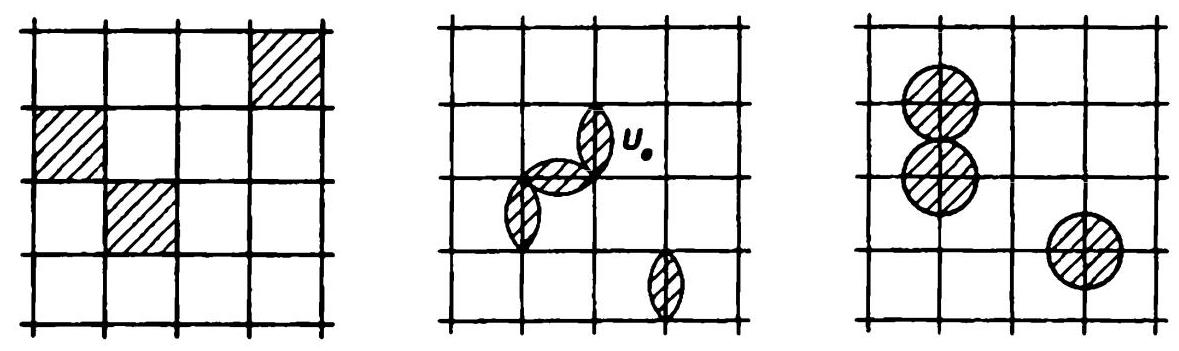
\includegraphics[width=1.0\textwidth]{images/50.1.jpg}
\end{center}
\hspace*{3em} 

Figure 50.1

Now let \(X\) be a compact subspace of \({\mathbb{R}}^{2}\;\) Given an open covering of \(X\) , it has a positive Lebesgue number \(\delta\) . Consider the homeomorphism \(f : {\mathbb{R}}^{2} \rightarrow  {\mathbb{R}}^{2}\) defined by the equation \(f\left( x\right)  = \left( {\delta /3}\right) x\) . The images under \(f\) of the open sets of the collection \(\mathcal{A}\) form an open covering of \({\mathbb{R}}^{2}\) by sets of diameter less than \(\delta\) , their intersections with \(X\) form the required open covering of \(X\) .

We shall generalize this result to compact subsets of \({\mathbb{R}}^{n}\) shortly.

Some basic facts about topological dimension are given in the following theorems:

\begin{theorem} Let \(X\) be a space having finite dimension. If \(Y\) is a closed subspace of \(X\) , then \(Y\) has finite dimension and \(\dim Y \leq  \dim X\) .
\end{theorem}

\begin{proof}Let \(\dim X = m\) . Let \(\mathcal{A}\) be a covering of \(Y\) by sets open in \(Y\) . For each \(A \in  \mathcal{A}\) , choose an open set \({A}^{\prime }\) of \(X\) such that \({A}^{\prime } \cap  Y = A\) . Cover \(X\) by the open sets \({A}^{\prime }\) , along with the open set \(X - Y\) . Let \(\mathcal{B}\) be a refinement of this covering that is an open covering of \(X\) and has order at most \(m + 1\) . Then the collection
\[
\{ B \cap  Y \mid  B \in  \mathcal{B}\}
\]

is a covering of \(Y\) by sets open in \(Y\) , it has order at most \(m + 1\) , and it refines \(\mathcal{A}\) .
\end{proof}
\begin{theorem} Let \(X = Y \cup  Z\) , where \(Y\) and \(Z\) are closed subspaces of \(X\) having finite topological dimension. Then

\[
\dim X = \max \{ \dim Y,\dim Z\} .
\]
\end{theorem}

\begin{proof}Let \(m = \max \{ \dim Y,\dim Z\}\) . We shall show that \(X\) is finite dimensional and has topological dimension at most \(m\) . It then follows from the preceding theorem that \(X\) has topological dimension precisely \(m\) .
Step 1. If \(\mathcal{A}\) is an open covering of \(X\) , we say that \(\mathcal{A}\) has order at most \(m + 1\) at points of \(Y\) provided no point of \(Y\) lies in more than \(m + 1\) elements of \(\mathcal{A}\) .

We show that if \(\mathcal{A}\) is an open covering of \(X\) , then there is an open covering of \(X\) that refines \(\mathcal{A}\) and has order at most \(m + 1\) at points of \(Y\) .

To prove this fact, consider the collection

\[
\{ A \cap  Y \mid  A \in  \mathcal{A}\} .
\]

It is an open covering of \(Y\) , so it has a refinement \(\mathcal{B}\) that is an open covering of \(Y\) and has order at most \(m + 1\) . Given \(B \in  \mathcal{B}\) , choose an open set \({U}_{B}\) of \(X\) such that \({U}_{B} \cap  Y = B\) . Choose also an element \({A}_{B}\) of \(\mathcal{A}\) such that \(B \subset  {A}_{B}\) . Let \(\mathcal{C}\) be the collection consisting of all the sets \({U}_{B} \cap  {A}_{B}\) , for \(B \in  \mathcal{B}\) , along with all the sets \(A - Y\) , for \(A \in  \mathcal{A}\) . Then \(\mathcal{C}\) is the desired open covering of \(X\) .

Step 2. Now let \(\mathcal{A}\) be an open covering of \(X\) . We construct an open covering \(\mathcal{D}\) of \(X\) that refines \(\mathcal{A}\) and has order at most \(m + 1\) . Let \(\mathcal{B}\) be an open covering of \(X\) refining \(\mathcal{A}\) that has order at most \(m + 1\) at points of \(Y\) . Then let \(\mathcal{C}\) be an open covering of \(X\) refining \(\mathcal{B}\) that has order at most \(m + 1\) at points of \(Z\) .

We form a new covering \(\mathcal{D}\) of \(X\) as follows: Define \(f : \mathcal{C} \rightarrow  \mathcal{B}\) by choosing for each \(C \in  \mathcal{C}\) an element \(f\left( C\right)\) of \(\mathcal{B}\) such that \(C \subset  f\left( C\right)\) . Given \(B \in  \mathcal{B}\) , define \(D\left( B\right)\) to be the union of all those elements \(C\) of \(\mathcal{C}\) for which \(f\left( C\right)  = B\) . (Of course, \(D\left( B\right)\) is empty if \(B\) is not in the image of \(f\) .) Let \(\mathcal{D}\) be the collection of all the sets \(D\left( B\right)\) , for \(B \in  \mathcal{B}\) .

Now \(\mathcal{D}\) refines \(\mathcal{B}\) , because \(D\left( B\right)  \subset  B\) for each \(B\) ; therefore, \(\mathcal{D}\) refines \(\mathcal{A}\) . Also, \(\mathcal{D}\) covers \(X\) because \(\mathcal{C}\) covers \(X\) and \(C \subset  D\left( {f\left( C\right) }\right)\) for each \(C \in  \mathcal{C}\) . We show that \(\mathcal{D}\) has order at most \(m + 1\) . Suppose \(x \in  D\left( {B}_{1}\right)  \cap  \cdots  \cap  D\left( {B}_{k}\right)\) , where the sets \(D\left( {B}_{i}\right)\) are distinct. We wish to prove that \(k \leq  m + 1\) . Note that the sets \({B}_{1},\ldots ,{B}_{k}\) must be distinct because the sets \(D\left( {B}_{i}\right)\) are. Because \(x \in  D\left( {B}_{i}\right)\) , we can choose for each \(i\) , a set \({C}_{i} \in  \mathcal{C}\) such that \(x \in  {C}_{i}\) and \(f\left( {C}_{i}\right)  = {B}_{i}\) . The sets \({C}_{i}\) are distinct because the sets \({B}_{i}\) are. Furthermore,

\[
x \in  \left\lbrack  {{C}_{1} \cap  \cdots  \cap  {C}_{k}}\right\rbrack   \subset  \left\lbrack  {D\left( {B}_{1}\right)  \cap  \cdots  \cap  D\left( {B}_{k}\right) }\right\rbrack   \subset  \left\lbrack  {{B}_{1} \cap  \cdots  \cap  {B}_{k}}\right\rbrack  .
\]

If \(x\) happens to lie in \(Y\) , then \(k \leq  m + 1\) because \(\mathcal{B}\) has order at most \(m + 1\) at points of \(Y\) ; and if \(x\) is in \(Z\) , then \(k \leq  m + 1\) because \(\mathcal{C}\) has order at most \(m + 1\) at points of \(z\) .
\end{proof}
\begin{corollary} Let \(X = {Y}_{1} \cup  \cdots  \cup  {Y}_{k}\) , where each \({Y}_{1}\) is a closed subspace of \(X\) and is finite dimensional. Then

\[
\dim X = \max \left\{  {\dim {Y}_{1},\ldots ,\dim {Y}_{k}}\right\}
\]
\end{corollary}
\end{example}

\begin{example} Every compact 1-manifold \(X\) has topological dimension 1. The space \(X\) can be written as a finite union of spaces that are homeomorphic to the unit interval \(\lbrack 0,1\}\) ; then the preceding corollary applies
\end{example}

\begin{example} Every compact 2-manifold \(X\) has topological dimension at most 2. The space \(X\) can be written as a finite union of spaces that are homeomorphic to the closed unit ball in \({\mathbb{R}}^{2}\) , then the preceding corollary applies.
\end{example}

An obvious question occurs at this point: Does a compact 2-manifold have topological dimension precisely 27 The answer is "yes," but the proof is not easy; it requires the tools of algebraic topology. We will prove in Part II of this book that every closed triangular region in \({\mathbb{R}}^{2}\) has topological dimension at least 2. (See §55.) It then follows that any compact subspace of \({\mathbb{R}}^{2}\) that contains a closed triangular region has topological dimension 2, from which it follows that every compact 2-manifold has topological dimension 2

\begin{example} An \idx{arc} \(A\) is a space homeomorphic to the closed unit interval; the end points of \(A\) are the points \(p\) and \(q\) such that \(A - \{ p\}\) and \(A - \{ q\}\) are connected \(A\) (finite) \idx{linear graph} \(G\) is a Hausdorff space that is written as the union of finitely many arcs, each pair of which intersect in at most a common end point. The arcs in the collection are called the edges of \(G\) , and the end points of the arcs are called the vertices of \(G\) Each edge of \(G\) , being compact, is closed in \(G\) ; the preceding corollary tells us that \(G\) has topological dimension 1
\end{example}

Two particular linear graphs are sketched in Figure 50.2. The first is a diagram of the familiar "gas-water-electricity problem"; the second is called the "complete graph on five vertices." Neither of them can be imbedded in \({\mathbb{R}}^{2}\) . Although this fact is "intuitively obvious," it is highly nontrivial to prove We shall give a proof in §64. are in \idx{general position} For if four of these points belonged to a single plane \({Ax} + {By} +\)  \({Cz} = D\) , then the polynomial equation

\[
{At} + B{t}^{2} + C{t}^{3} = D
\]

\begin{center}
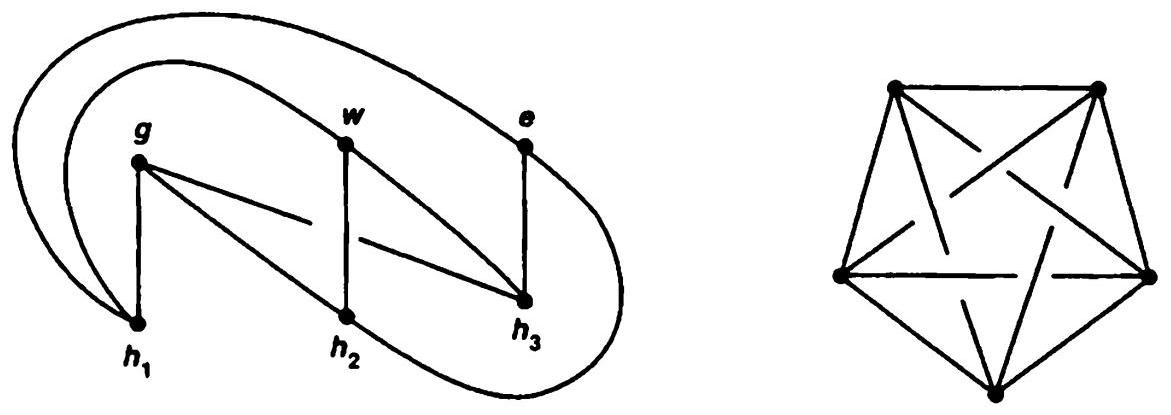
\includegraphics[width=1.0\textwidth]{images/50.2.jpg}
\end{center}
\hspace*{3em} 

Figure 50.2

\begin{example} Every finite linear graph can be imbedded in \({\mathbb{R}}^{3}\) . The proof involves the notion of "general position." A set \(S\) of points of \({\mathbb{R}}^{3}\) is said to be in general posinon if no three of the points of \(S\) are collinear and no four of them are coplanar. It is easy to find such a set of points. For example, the points of the curve

\[
S = \left\{  {\left( {t,{t}^{2},{t}^{3}}\right)  \mid  t \in  \mathbb{R}}\right\}
\]

would have four distinct real roots \({}^{1}\) And if three of these points belonged to a single line, we could take an additional point of \(S\) and obtain four points that lie on a plane.

Now, given a finite linear graph \(G\) , with vertices \({v}_{1},\ldots ,{v}_{n}\) , let us choose a set \(\left\{  {{\mathbf{z}}_{1},\ldots ,{\mathbf{z}}_{n}}\right\}\) of points of \({\mathbb{R}}^{3}\) that is in general position. Define a map \(f : G \rightarrow  {\mathbb{R}}^{3}\) by letting \(f\) map the vertex \({v}_{i}\) to the point \({\mathbf{z}}_{i}\) , and map the edge joining \({v}_{i}\) and \({v}_{j}\) homeo-morphically onto the line segment joining \({\mathbf{z}}_{i}\) and \({\mathbf{z}}_{j}\) . Now each edge of \(G\) is closed in \(G\) It follows that \(f\) is continuous, by the pasting lemma. We show that \(f\) is injective, from which it follows that \(f\) is an imbedding. Let \(e = {v}_{i}{v}_{j}\) and \({e}^{\prime } = {v}_{k}{v}_{m}\) be two edges of \(G\) If they have no vertex in common, then the line segments \(f\left( e\right)\) and \(f\left( {e}^{\prime }\right)\) are disjoint, for otherwise the points \({\mathbf{z}}_{i},{\mathbf{z}}_{j},{\mathbf{z}}_{k},{\mathbf{z}}_{m}\) would be coplanar. And if \(e\) and \({e}^{\prime }\) have a vertex in common, so that \(i = k\) , say, then the line segments \(f\left( e\right)\) and \(f\left( {e}^{\prime }\right)\) intersect only in the point \({\mathbf{z}}_{i} = {\mathbf{z}}_{k}\) , for otherwise \({\mathbf{z}}_{i},{\mathbf{z}}_{j}\) , and \({\mathbf{z}}_{m}\) would be collinear.
\end{example}

Now we prove our general imbedding theorem, to the effect that every compact metrizable space of topological dimension \(m\) can be imbedded in \({\mathbb{R}}^{{2m} + 1}\) . This theorem is another "deep" theorem; it is not at all obvious, for instance, why \({2m} + 1\) should be the crucial dimension. That will come out in the course of the proof.

To prove the imbedding theorem, we shall need to generalize the notion of general position to \({\mathbb{R}}^{N}\) . This involves a bit of the analytic geometry of \({\mathbb{R}}^{N}\) , which is nothing more than the usual linear algebra of \({\mathbb{R}}^{N}\) translated into somewhat different language.

\begin{definition} A set \(\left\{  {{\mathbf{x}}_{0},\ldots ,{\mathbf{x}}_{k}}\right\}\) of points of \({\mathbb{R}}^{N}\) is said to be \idx{geometrically independent}, or \idx{affinely independent}, if the equations

\[
\mathop{\sum }\limits_{{i = 0}}^{k}{a}_{i}{\mathbf{x}}_{i} = \mathbf{0}\;\text{ and }\;\mathop{\sum }\limits_{{i = 0}}^{k}{a}_{i} = 0
\]

hold only if each \({a}_{t} = 0\) .
\end{definition}

Obviously, a set consisting of only one point is geometrically independent. But what does geometric independence mean in general? If we solve the second equation for \({a}_{0}\) and plug the answer into the first equation, we see that this definition is equivalent to the statement that the equation

\[
\mathop{\sum }\limits_{{i = 1}}^{k}{a}_{i}\left( {{\mathbf{x}}_{i} - {\mathbf{x}}_{0}}\right)  = \mathbf{0}
\]

holds only if each \({a}_{i} = 0\) . This is just the definition of linear independence for the set of vectors \({\mathbf{x}}_{1} - {\mathbf{x}}_{0},\ldots ,{\mathbf{x}}_{k} - {\mathbf{x}}_{0}\) of the vector space \({\mathbb{R}}^{N}\) . This gives us something to visualize: Any two distinct points form a geometrically independent set. Three points form a geometrically independent set if they are not collinear. Four points in \({\mathbb{R}}^{3}\) form a geometrically independent set if they are not coplanar. And so on.

It follows from these remarks that the points

\[
\mathbf{0} = \left( {0,0,\ldots ,0}\right) \text{ , }
\]

\[
{\epsilon }_{1} = \left( {1,0,\ldots ,0}\right) \text{ , }
\]

\[
{\epsilon }_{N} = \left( {0,0,\ldots ,1}\right)
\]

are geometrically independent in \({\mathbb{R}}^{N}\) . It also follows that any geometrically independent set of points in \({\mathbb{R}}^{N}\) contains no more than \(N + 1\) points

\begin{definition} Let \(\left\{  {{\mathbf{x}}_{0},\ldots ,{\mathbf{x}}_{k}}\right\}\) be a set of points of \({\mathbb{R}}^{N}\) that is geometrically independent. The plane \(P\) determined by these points is defined to be the set of all points \(\mathbf{x}\) of \({\mathbb{R}}^{N}\) such that

\[
\mathbf{x} = \mathop{\sum }\limits_{{i = 0}}^{k}{t}_{i}{\mathbf{x}}_{i},\;\text{ where }\mathop{\sum }\limits_{{i = 0}}^{k}{t}_{i} = 1.
\]
\end{definition}

It is simple algebra to check that \(P\) can also be expressed as the set of all points \(\mathbf{x}\) such that

(*)
\[
\mathbf{x} = {\mathbf{x}}_{0} + \mathop{\sum }\limits_{{i = 1}}^{k}{a}_{i}\left( {{\mathbf{x}}_{i} - {\mathbf{x}}_{0}}\right)
\]

for some scalars \({a}_{1},\ldots ,{a}_{k}\) . Thus \(P\) can be described not only as "the plane determined by the points \({\mathbf{x}}_{0},\ldots ,{\mathbf{x}}_{k}\) ," but also as "the plane passing through the point \({\mathbf{x}}_{0}\) parallel to the vectors \({\mathbf{x}}_{1} - {\mathbf{x}}_{0},\ldots ,{\mathbf{x}}_{k} - {\mathbf{x}}_{0}\) ."

Consider now the homeomorphism \(T : {\mathbb{R}}^{N} \rightarrow  {\mathbb{R}}^{N}\) defined by the equation \(T\left( \mathbf{x}\right)  = \mathbf{x} - {\mathbf{x}}_{0}\) . It is called a translation of \({\mathbb{R}}^{N}\) . Expression (*) shows that this map carries the plane \(P\) onto the vector subspace \({V}^{k}\) of \({\mathbb{R}}^{N}\) having as basis the vectors \({\mathbf{x}}_{1} - {\mathbf{x}}_{0},\ldots ,{\mathbf{x}}_{k} - {\mathbf{x}}_{0}\) . For this reason, we often call \(P\) a \(k\) -plane in \({\mathbb{R}}^{N}\) .

Two facts follow at once: First, if \(k < N\) , the \(k\) -plane \(P\) necessarily has empty interior in \({\mathbb{R}}^{N}\) (because \({V}^{k}\) does). And second, if \(\mathbf{y}\) is any point of \({\mathbb{R}}^{N}\) not lying in \(P\) , then the set

\[
\left\{  {{\mathbf{x}}_{0},\ldots ,{\mathbf{x}}_{k},\mathbf{y}}\right\}
\]

is geometrically independent. For if \(\mathbf{y} \notin  P\) , then \(T\left( \mathbf{y}\right)  = \mathbf{y} - {\mathbf{x}}_{0}\) is not in \({V}^{k}\) . By a standard theorem of linear algebra, the vectors \(\left\{  {{\mathbf{x}}_{1} - {\mathbf{x}}_{0},\ldots ,{\mathbf{x}}_{k} - {\mathbf{x}}_{0},\mathbf{y} - {\mathbf{x}}_{0}}\right\}\) are linearly independent, from which our result follows.

\begin{definition} A set \(A\) of points of \({\mathbb{R}}^{N}\) is said to be in general position in \({\mathbb{R}}^{N}\) if every subset of \(A\) containing \(N + 1\) or fewer points is geometrically independent.
\end{definition}

In the case of \({\mathbb{R}}^{3}\) , this is the same as the definition given earlier, as you can check.

\begin{lemma} Given a finite set \(\left\{  {{\mathbf{x}}_{1},\ldots ,{\mathbf{x}}_{n}}\right\}\) of points of \({\mathbb{R}}^{N}\) and given \(\delta  > 0\) , there exists a set \(\left\{  {{\mathbf{y}}_{1},\ldots ,{\mathbf{y}}_{n}}\right\}\) of points of \({\mathbb{R}}^{N}\) in general position in \({\mathbb{R}}^{N}\) , such that \(\left| {{\mathbf{x}}_{i} - {\mathbf{y}}_{i}}\right|  < \delta\) for all \(i\) .
\end{lemma}

\begin{proof}We proceed by induction. Set \({\mathbf{y}}_{1} = {\mathbf{x}}_{1}\) . Suppose that we are given \({\mathbf{y}}_{1},\ldots ,{\mathbf{y}}_{p}\) in general position in \({\mathbb{R}}^{N}\) . Consider the set of all planes in \({\mathbb{R}}^{N}\) determined by subsets of \(\left\{  {{\mathbf{y}}_{1},\ldots ,{\mathbf{y}}_{p}}\right\}\) that contain \(N\) or fewer elements. Every such subset is geometrically independent and determines a \(k\) -plane of \({\mathbb{R}}^{N}\) for some \(k \leq  N - 1\) . Each of these planes has empty interior in \({\mathbb{R}}^{N}\) Because there are only finitely many of them, their union also has empty interior in \({\mathbb{R}}^{N}\) . (Recall that \({\mathbb{R}}^{N}\) is a Bare space.) Choose \({\mathbf{y}}_{p + 1}\) to be a point of \({\mathbb{R}}^{N}\) within \(\delta\) of \({\mathbf{x}}_{p + 1}\) that does not lie in any of these planes. It follows at once that the set
\[
C = \left\{  {{\mathbf{y}}_{1},\ldots ,{\mathbf{y}}_{p},{\mathbf{y}}_{p + 1}}\right\}
\]

is in general position in \({\mathbb{R}}^{N}\) . For let \(D\) be any subset of \(C\) containing \(N + 1\) or fewer elements. If \(D\) does not contain \({\mathbf{y}}_{p + 1}\) , then \(D\) is geometrically independent by the induction hypothesis. If \(D\) does contain \({\mathbf{y}}_{p + 1}\) , then \(D - \left\{  {\mathbf{y}}_{p + 1}\right\}\) contains \(N\) or fewer points and \({\mathbf{y}}_{p + 1}\) is not in the plane determined by these points, by construction. Then as noted above, \(D\) is geometrically independent.
\end{proof}
\begin{theorem}[The imbedding theorem] Every compact metrizable space \(X\) of topological dimension \(m\) can be imbedded in \({\mathbb{R}}^{{2m} + 1}\) .
\end{theorem}

\begin{proof}Let \(N = {2m} + 1\) . Let us denote the square metric for \({\mathbb{R}}^{N}\) by
\[
\left| {\mathbf{x} - \mathbf{y}}\right|  = \max \left\{  {\left| {{x}_{i} - {y}_{i}}\right| ;i = 1,\ldots ,N}\right\}  .
\]

Then we can use \(\rho\) to denote the corresponding sup metric on the space \(\mathcal{C}\left( {X,{\mathbb{R}}^{N}}\right)\) ;

\[
\rho \left( {f,g}\right)  = \sup \{ \left| {f\left( x\right)  - g\left( x\right) }\right| ,x \in  X\} .
\]

The space \(\mathcal{C}\left( {X,{\mathbb{R}}^{N}}\right)\) is complete in the metric \(\rho\) , since \({\mathbb{R}}^{N}\) is complete in the square metric

Choose a metric \(d\) for the space \(X\) ; because \(X\) is compact, \(d\) is bounded. Given a continuous map \(f : X \rightarrow  {\mathbb{R}}^{N}\) , let us define

\[
\Delta \left( f\right)  = \sup \left\{  {\operatorname{diam}{f}^{-1}\left( {\{ z\} }\right)  \mid  z \in  f\left( X\right) }\right\}  .
\]

The number \(\Delta \left( f\right)\) measures how far \(f\) "deviates" from being injective; if \(\Delta \left( f\right)  = 0\) , each set \({f}^{-1}\left( {\{ z\} }\right)\) consists of exactly one point, so \(f\) is injective.

Now, given \(\epsilon  > 0\) , define \({U}_{\epsilon }\) to be the set of all those continuous maps \(f : X \rightarrow\)  \({\mathbb{R}}^{N}\) for which \(\Delta \left( f\right)  < \epsilon\) ; it consists of all those maps that "deviate" from being injective by less than \(\epsilon\) . We shall show that \({U}_{\epsilon }\) is both open and dense in \(\mathcal{C}\left( {X,{\mathbb{R}}^{N}}\right)\) . It follows that the intersection

\[
\mathop{\bigcap }\limits_{{n \in  {\mathbf{Z}}_{ + }}}{U}_{1/n}
\]

is dense in \(\mathcal{C}\left( {X,{\mathbb{R}}^{N}}\right)\) and is in particular nonempty.

If \(f\) is an element of this intersection, then \(\Delta \left( f\right)  < 1/n\) for every \(n\) . Therefore, \(\Delta \left( f\right)  = 0\) and \(f\) is injective. Because \(X\) is compact, \(f\) is an imbedding. Thus, the imbedding theorem is proved.

(1) \({U}_{\epsilon }\) is open in \(\mathcal{C}\left( {X,{\mathbb{R}}^{N}}\right)\) . Given an element \(f\) of \({U}_{\epsilon }\) , we wish to find some ball \({B}_{\rho }\left( {f,\delta }\right)\) about \(f\) that is contained in \({U}_{\epsilon }\) . First choose a number \(b\) such that \(\Delta \left( f\right)  < b < \epsilon\) . Note that if \(f\left( x\right)  = f\left( y\right)  = z\) , then \(x\) and \(y\) belong to the set \({f}^{-1}\left( {\{ z\} }\right)\) , so that \(d\left( {x,y}\right)\) must be less than \(b\) It follows that if we let \(A\) be the following subset of \(X \times  X\) ,

\[
A = \{ x \times  y \mid  d\left( {x,y}\right)  \geq  b\}
\]

then the function \(\left| {f\left( x\right)  - f\left( y\right) }\right|\) is positive on \(A\) . Now \(A\) is closed in \(X \times  X\) and therefore compact; hence the function \(\left| {f\left( x\right)  - f\left( y\right) }\right|\) has a positive minimum on \(A\) . Let

\[
\delta  = \frac{1}{2}\min \{ \left| {f\left( x\right)  - f\left( y\right) }\right| ;x \times  y \in  A\} .
\]

We assert that this value of \(\delta\) will suffice.

Suppose that \(g\) is a map such that \(\rho \left( {f,g}\right)  < \delta\) . If \(x \times  y \in  A\) , then \(\left| {f\left( x\right)  - f\left( y\right) }\right|  \geq\)  \({2\delta }\) by definition; since \(g\left( x\right)\) and \(g\left( y\right)\) are within \(\delta\) of \(f\left( x\right)\) and \(f\left( y\right)\) , respectively, we must have \(\left| {g\left( x\right)  - g\left( y\right) }\right|  > 0\) . Hence the function \(\left| {g\left( x\right)  - g\left( y\right) }\right|\) is positive on \(A\) . As a result, if \(x\) and \(y\) are two points such that \(g\left( x\right)  = g\left( y\right)\) , then necessarily \(d\left( {x,y}\right)  < b\) . We conclude that \({\Delta g} \leq  b < \epsilon\) , as desired.

(2) \({U}_{\epsilon }\) is dense in \(\mathcal{C}\left( {X,{\mathbb{R}}^{N}}\right)\) . This is the difficult part of the proof. We need to use the analytic geometry of \({\mathbb{R}}^{N}\) discussed earlier. Let \(f \in  \mathcal{C}\left( {X,{\mathbb{R}}^{N}}\right)\) . Given \(\epsilon  > 0\) and given \(\delta  > 0\) , we wish to find a function \(g \in  \mathcal{C}\left( {X,{\mathbb{R}}^{N}}\right)\) such that \(g \in  {U}_{\epsilon }\) and \(\rho \left( {f,g}\right)  < \delta\) .

Let us cover \(X\) by finitely many open sets \(\left\{  {{U}_{1},\ldots ,{U}_{n}}\right\}\) such that

(1) \(\operatorname{diam}{U}_{i} < \epsilon /2\) in \(X\) ,

(2) \(\operatorname{diam}f\left( {U}_{i}\right)  < \delta /2\) in \({\mathbb{R}}^{N}\) ,

(3) \(\left\{  {{U}_{1},\ldots ,{U}_{n}}\right\}\) has order \(\leq  m + 1\) .

Let \(\left\{  {\phi }_{i}\right\}\) be a partition of unity dominated by \(\left\{  {U}_{i}\right\}\) (see \(§{36}\) ). For each \(i\) , choose a point \({x}_{i} \in  {U}_{i}\) . Then choose, for each \(i\) , a point \({\mathbf{z}}_{i} \in  {\mathbb{R}}^{N}\) such that \({\mathbf{z}}_{i}\) is within \(\delta /2\) of the point \(f\left( {x}_{i}\right)\) , and such that the set \(\left\{  {{\mathbf{z}}_{1},\ldots ,{\mathbf{z}}_{n}}\right\}\) is in general position in \({\mathbb{R}}^{N}\) . Finally, define \(g : X \rightarrow  {\mathbb{R}}^{N}\) by the equation

\[
g\left( x\right)  = \mathop{\sum }\limits_{{i = 1}}^{n}{\phi }_{i}\left( x\right) {\mathbf{z}}_{i}.
\]

We assert that \(g\) is the desired function.

First, we show that \(\rho \left( {f,g}\right)  < \delta\) . Note that

\[
g\left( x\right)  - f\left( x\right)  = \mathop{\sum }\limits_{{i = 1}}^{n}{\phi }_{i}\left( x\right) {\mathbf{z}}_{i} - \mathop{\sum }\limits_{{i = 1}}^{n}{\phi }_{i}\left( x\right) f\left( x\right) ;
\]

here we use the fact that \(\sum {\phi }_{i}\left( x\right)  = 1\) Then

\[
g\left( x\right)  - f\left( x\right)  = \sum {\phi }_{i}\left( x\right) \left( {{\mathbf{z}}_{i} - f\left( {x}_{i}\right) }\right)  + \sum {\phi }_{i}\left( x\right) \left( {f\left( {x}_{i}\right)  - f\left( x\right) }\right) .
\]

Now \(\left| {{\mathbf{z}}_{i} - f\left( {x}_{i}\right) }\right|  < \delta /2\) for each \(i\) , by choice of the points \({\mathbf{z}}_{i}\) . And if \(i\) is an index such that \({\phi }_{i}\left( x\right)  \neq  0\) , then \(x \in  {U}_{i}\) ; because we have diam \(f\left( {U}_{i}\right)  < \delta /2\) , it follows that \(\left| {f\left( {x}_{i}\right)  - f\left( x\right) }\right|  < \delta /2\) . Since \(\sum {\phi }_{i}\left( x\right)  = 1\) , we conclude that \(\left| {g\left( x\right)  - f\left( x\right) }\right|  < \delta\) . Therefore, \(\rho \left( {g,f}\right)  < \delta\) , as desired.

Second, we show that \(g \in  {U}_{\epsilon }\) . We shall prove that if \(x,y \in  X\) and \(g\left( x\right)  = g\left( y\right)\) , then \(x\) and \(y\) belong to one of the open sets \({U}_{i}\) , so that necessarily \(d\left( {x,y}\right)  < \epsilon /2\) (since \(\operatorname{diam}{U}_{i} < \epsilon /2\) ). As a result, \(\Delta \left( g\right)  \leq  \epsilon /2 < \epsilon\) , as desired.

So suppose \(g\left( x\right)  = g\left( y\right)\) . Then

\[
\mathop{\sum }\limits_{{i = 1}}^{n}\left\lbrack  {{\phi }_{i}\left( x\right)  - {\phi }_{i}\left( y\right) }\right\rbrack  {\mathbf{z}}_{i} = \mathbf{0}.
\]

Because the covering \(\left\{  {U}_{i}\right\}\) has order at most \(m + 1\) , at most \(m + 1\) of the numbers \({\phi }_{i}\left( x\right)\) are nonzero, and at most \(m + 1\) of the numbers \({\phi }_{i}\left( y\right)\) are nonzero. Thus, the sum \(\sum \left\lbrack  {{\phi }_{i}\left( x\right)  - {\phi }_{i}\left( y\right) }\right\rbrack  {\mathbf{z}}_{i}\) has at most \({2m} + 2\) nonzero terms. Note that the sum of the coefficients vanishes because

\[
\sum \left\lbrack  {{\phi }_{i}\left( x\right)  - {\phi }_{i}\left( y\right) }\right\rbrack   = 1 - 1 = 0.
\]

The points \({\mathbf{z}}_{i}\) are in general position in \({\mathbb{R}}^{N}\) , so that any subset of them having \(N + 1\) or fewer elements is geometrically independent. And by hypothesis \(N + 1 = {2m} + 2\) . (Aha!) Therefore, we conclude that

\[
{\phi }_{i}\left( x\right)  - {\phi }_{i}\left( y\right)  = 0
\]

for all \(i\) .

Now \({\phi }_{i}\left( x\right)  > 0\) for some \(i\) , so that \(x \in  {U}_{i}\) . Since \({\phi }_{i}\left( y\right)  = {\phi }_{i}\left( x\right)\) , we have \(y \in  {U}_{i}\) also, as asserted.

To give some content to the imbedding theorem, we need some more examples of spaces that are finite dimensional. We prove the following theorem.
\end{proof}
\begin{theorem} Every compact subspace of \({\mathbb{R}}^{N}\) has topological dimension at most \(N\) .
\end{theorem}

Proof The proof is a generalization of the proof given in Example 3 for \({\mathbb{R}}^{2}\) . Let \(\rho\) be the square metric on \({\mathbb{R}}^{N}\) .

Step 1. We begin by breaking \({\mathbb{R}}^{N}\) up into "unit cubes." Define \(\mathcal{J}\) to be the following collection of open intervals in \(\mathbb{R}\) :

\[
g = \{ \left( {n,n + 1}\right)  \mid  n \in  \mathbb{Z}\}
\]

and define \(\mathcal{K}\) to be the following collection of one-point sets in \(\mathbb{R}\) :

\[
\mathcal{K} = \{ \{ n\}  \mid  n \in  \mathbb{Z}\}
\]

If \(M\) is an integer such that \(0 \leq  M \leq  N\) , let \({\mathcal{C}}_{M}\) denote the set of all products

\[
C = {A}_{1} \times  {A}_{2} \times   \cdot   \times  {A}_{N},
\]

where exactly \(M\) of the sets \({A}_{i}\) belong to \(\mathcal{J}\) , and the remainder belong to \(\mathcal{K}\) . If \(M > 0\) , then \(C\) is homeomorphic to the product \({\left( 0,1\right) }^{M}\) and will be called an \(M\) -cube. If \(M = 0\) , then \(C\) consists of a single point and will be called a 0 -cube

Let \(\mathcal{C} = {\mathcal{C}}_{0} \cup  {\mathcal{C}}_{1} \cup   \cdot   \cup  {\mathcal{C}}_{N}\) . Note that each point \(\mathbf{x}\) of \({\mathbb{R}}^{N}\) lies in precisely one element of \(\mathcal{C}\) because each real number \({x}_{i}\) lies in precisely one element of \(\mathcal{J} \cup  \mathcal{K}\) . We shall expand each element \(C\) of \(\mathcal{C}\) slightly to an open set \(U\left( C\right)\) of \({\mathbb{R}}^{N}\) of diameter at most \(3/2\) , in such a way that if \(C\) and \(D\) are two different \(M\) -cubes, then \(U\left( C\right)\) and \(U\left( D\right)\) are disjoint.

Let \(\mathbf{x} = \left( {{x}_{1},\ldots ,{x}_{N}}\right)\) be a point of the \(M\) -cube \(C\) . We show that there is a number \(\epsilon \left( \mathbf{x}\right)  > 0\) such that the \(\epsilon \left( \mathbf{x}\right)\) -neighborhood of \(\mathbf{x}\) intersects no \(M\) -cube other than \(C\) . If \(C\) is a 0 -cube, we set \(\epsilon \left( \mathbf{x}\right)  = 1/2\) and we are finished. Otherwise, \(M > 0\) , and exactly \(M\) of the numbers \({x}_{i}\) are not integers. Choose \(\epsilon  \leq  1/2\) so that for each \({x}_{i}\) that is not an integer, the interval \(\left( {{x}_{i} - \epsilon ,{x}_{i} + \epsilon }\right)\) contains no integer. If \(\mathbf{y} = \left( {{y}_{1},\ldots ,{y}_{N}}\right)\) is a point lying in the \(\epsilon\) -neighborhood of \(\mathbf{x}\) , then \({y}_{i}\) is nonintegral whenever \({x}_{i}\) is nonintegral. This means that \(y\) either belongs to the same \(M\) -cube as \(x\) does, or \(y\) belongs to some \(L\) -cube for \(L > M\) . In either case, the \(\epsilon\) -neighborhood of \(\mathbf{x}\) intersects no \(M\) -cube other than \(C\) .

Given an \(M\) -cube \(C\) , we define the neighborhood \(U\left( C\right)\) of \(C\) to be the union of the \(\epsilon \left( \mathbf{x}\right) /2\) -neighborhoods of \(\mathbf{x}\) for all \(\mathbf{x} \in  C\) It is then immediate that if \(C\) and \(D\) are different \(M\) -cubes, \(U\left( C\right)\) and \(U\left( D\right)\) are disjoint. Furthermore, if \(\mathbf{z}\) is a point of \(U\left( C\right)\) , then \(d\left( {\mathbf{z},\mathbf{x}}\right)  < \epsilon \left( \mathbf{x}\right) /2 < 1/4\) for some point \(\mathbf{x}\) of \(C\) . Since \(C\) has diameter 1, the set \(U\left( C\right)\) has diameter at most \(3/2\) .

Step 2. Given \(M\) with \(0 \leq  M \leq  N\) , define \({\mathcal{A}}_{M}\) to be the collection of all sets \(U\left( C\right)\) , where \(C \in  {\mathcal{C}}_{M}\) . The elements of \({\mathcal{A}}_{M}\) are disjoint, and each has diameter at most \(3/2\) . The remainder of the proof is a copy of the proof given in Example 3 for \({\mathbb{R}}^{2}\) .

\begin{corollary} Every compact \(m\) -manifold has topological dimension at most \(m\)
\end{corollary}

\begin{corollary} Every compact \(m\) -manifold can be imbedded in \({\mathbb{R}}^{{2m} + 1}\) .
\end{corollary}

\begin{corollary} Let \(X\) be a compact metrizable space. Then \(X\) can be imbedded in some euclidean space \({\mathbb{R}}^{N}\) if and only if \(X\) has finite topological dimension.
\end{corollary}

As mentioned earlier, much of what we have proved holds without assumption of compactness. We ask you to prove the appropriate generalizations in the exercises that follow

One thing we do not ask you to prove is the fact that the topological dimension of an \(m\) -manifold is precisely \(m\) . And for good reason; the proof requires the tools of algebraic topology.

Nor do we ask you to prove that \(N = {2m} + 1\) is the smallest value of \(N\) such that every compact metrizable space of topological dimension \(m\) can be imbedded in \({\mathbb{R}}^{N}\) . The reason is the same. Even in the case of a linear graph, where \(m = 1\) , the proof is nontrivial, as we remarked earlier.

For further results in dimension theory, the reader is referred to the classical book of Hurewicz and Wallman 		\cite{HurewiczWallman1974}. In particular, this book discusses another, entirely different, definition of topological dimension, due to Menger and Urysohn. It is an \idx{Inductive dimension} inductive definition. The empty set has dimension -1 . And a space has dimension at most \(n\) if there is a basis for its topology such that for each basis element \(B\) , the boundary of \(B\) has dimension at most \(n - 1\) The dimension of a space is the smallest value of \(n\) for which this condition holds. This notion of dimension agrees with ours for compact metrizable spaces.

\section*{Exercises}

1. Show that any discrete space has dimension 0

2. Show that any connected \({T}_{1}\) space having more than one point has dimension at least 1.

3. Show that the topologist's sine curve has dimension 1.

4. Show that the points \(0,{\epsilon }_{1},{\epsilon }_{2},{\epsilon }_{3}\) , and(1,1,1)are in general position in \({\mathbb{R}}^{3}\) . Sketch the corresponding imbedding into \({\mathbb{R}}^{3}\) of the complete graph on five vertices.

5. Examine the proof of the imbedding theorem in the case \(m = 1\) and show that the map \(g\) of part (2) actually maps \(X\) onto a linear graph in \({\mathbb{R}}^{3}\) .

6. Prove the following:

\begin{theorem} Let \(X\) be a locally compact Hausdorff space with a countable basis, such that every compact subspace of \(X\) has topological dimension at most \(m\) . Then \(X\) is homeomorphic to a closed subspace of \({\mathbb{R}}^{{2m} + 1}\) .
\end{theorem}

\begin{proof}If \(f : X \rightarrow  {\mathbb{R}}^{N}\) is a continuous map, we say \(f\left( x\right)  \rightarrow  \infty\) as \(x \rightarrow  \infty\) if given \(n\) , there is a compact subspace \(C\) of \(X\) such that \(f\left( x\right)  > n\) for \(x \in  X - C\) .
(a) Let \(\bar{\rho }\) be the uniform metric on \(\mathcal{C}\left( {X,{\mathbb{R}}^{N}}\right)\) . Show that if \(f\left( x\right)  \rightarrow  \infty\) as \(x \rightarrow  \infty\) and \(\bar{\rho }\left( {f,g}\right)  < 1\) , then \(g\left( x\right)  \rightarrow  \infty\) as \(x \rightarrow  \infty\) .

(b) Show that if \(f\left( x\right)  \rightarrow  \infty\) as \(x \rightarrow  \infty\) , then \(f\) extends to a continuous map of one-point compactifications. Conclude that if \(f\) is injective as well, then \(f\) is a homeomorphism of \(X\) with a closed subspace of \({\mathbb{R}}^{N}\) .

(c) Given \(f : X \rightarrow  {\mathbb{R}}^{N}\) and given a compact subspace \(C\) of \(X\) , let

\[
{U}_{\epsilon }\left( C\right)  = \{ f \mid  \Delta \left( {f \mid  C}\right)  < \epsilon \} .
\]

Show that \({U}_{\epsilon }\left( C\right)\) is open in \(\mathcal{C}\left( {X,{\mathbb{R}}^{N}}\right)\) .

(d) Show that if \(N = {2m} + 1\) , then \({U}_{\epsilon }\left( C\right)\) is dense in \(\mathcal{C}\left( {X,{\mathbb{R}}^{N}}\right)\) . [Hint Given \(f\) and given \(\epsilon ,\delta  > 0\) , choose \(g : C \rightarrow  {\mathbb{R}}^{N}\) so that \(d\left( {f\left( x\right) ,g\left( x\right) }\right)  < \delta\) for \(x \in  C\) , and \(\Delta \left( g\right)  < \epsilon\) . Extend \(f - g\) to \(h : X \rightarrow  {\left\lbrack  -\delta ,\delta \right\rbrack  }^{N}\) using the Tietze theorem.]

(e) Show there exists a map \(f : X \rightarrow  \mathbb{R}\) such that \(f\left( x\right)  \rightarrow  \infty\) as \(x \rightarrow  \infty\) . [Hint: Write \(X\) as the union of compact subspaces \({C}_{n}\) such that \({C}_{n} \subset\) Int \({C}_{n + 1}\) for each \(n\) .]

(f) Let \({C}_{n}\) be as in (e). Use the fact that \(\bigcap {U}_{1/n}\left( {C}_{n}\right)\) is dense in \(\mathcal{C}\left( {X,{\mathbb{R}}^{N}}\right)\) to complete the proof.

7. Corollary. Every \(m\) -manifold can be imbedded in \({\mathbb{R}}^{{2m} + 1}\) as a closed subspace.

8. Recall that \(X\) is said to be \(\sigma\) -compact if there is a countable collection of compact subspaces of \(X\) whose interiors cover \(X\)

\begin{theorem} Let \(X\) be a \(\sigma\) -compact Hausdorff space. If every compact subspace of \(X\) has topological dimension at most \(m\) , then so does \(X\) .
\end{theorem}

Proof. Let \(\mathcal{A}\) be an open cover of \(X\) . Find an open cover \(\mathcal{B}\) of \(X\) refining \(\mathcal{A}\) that has order at most \(m + 1\) , as follows:

(a) Show that \(X = \bigcup {X}_{n}\) , where \({X}_{n}\) is compact and \({X}_{n} \subset  \operatorname{Int}{X}_{n + 1}\) for each \(n\) . Let \({X}_{0} = \varnothing\) .

(b) Find an open covering \({\mathcal{B}}_{0}\) of \(X\) refining \(\mathcal{A}\) such that for each \(n\) , each element of \({\mathcal{B}}_{0}\) that intersects \({X}_{n}\) lies in \({X}_{n + 1}\) .

(c) Suppose \(n \geq  0\) and \({\mathcal{B}}_{n}\) is an open covering of \(X\) refining \({\mathcal{B}}_{0}\) such that \({\mathcal{B}}_{n}\) has order at most \(m + 1\) at points of \({X}_{n}\) . Choose an open covering \(\mathcal{C}\) of \(X\) refining \({\mathcal{B}}_{n}\) that has order at most \(m + 1\) at points of \({X}_{n + 1}\) . Choose \(f.\mathcal{C} \rightarrow  {\mathcal{B}}_{n}\) so that \(C \subset  f\left( C\right)\) . For \(B \in  {\mathcal{B}}_{n}\) , let \(D\left( B\right)\) be the union of those \(C\) for which \(f\left( C\right)  = B\) . Let \({\mathcal{B}}_{n + 1}\) consist of all sets \(B \in  {\mathcal{B}}_{n}\) for which \(B \cap  {X}_{n - 1} \neq  \varnothing\) , along with all sets \(D\left( B\right)\) for which \(B \in  {\mathcal{B}}_{n}\) and \(B \cap  {X}_{n - 1} = \varnothing\) . Show that \({\mathcal{B}}_{n + 1}\) is an open covering of \(X\) that refines \({\mathcal{B}}_{n}\) and has order at most \(m + 1\) at points of \({X}_{n + 1}\) .

(d) Define \(\mathcal{B}\) as follows: Given a set \(B\) , it belongs to \(\mathcal{B}\) if there is an \(N\) such that \(B \in  {\mathcal{B}}_{n}\) for all \(n \geq  N\) .

9. Corollary. Every \(m\) -manifold has topological dimension at most \(m\) .

10. Corollary. Every closed subspace of \({\mathbb{R}}^{N}\) has topological dimension at most \(N\) .

11. Corollary. A space \(X\) can be imbedded as a closed subspace of \({\mathbb{R}}^{N}\) for some \(N\) if and only if \(X\) is locally compact and Hausdorff with a countable basis, and has finite topological dimension.
\end{proof}
\section*{* Supplementary Exercises: Locally Euclidean Spaces}

A space \(X\) is said to be locally m-euclidean if for each \(x \in  X\) , there is a neighborhood of \(x\) that is homeomorphic to an open set of \({\mathbb{R}}^{m}\) . Such a space \(X\) automatically satisfies the \({T}_{1}\) axiom, but it need not be Hausdorff. (See the exercises of \(§{36}\) .) However, if \(X\) is Hausdorff and has a countable basis, then \(X\) is called an \(m\) -manifold.

Throughout these exercises, let \(X\) be a space that is locally \(m\) -euclidean.

1. Show that \(X\) is locally compact and locally metrizable.

2. Consider the following conditions on \(X\) :

(i) \(X\) is compact Hausdorff.

(ii) \(X\) is an \(m\) -manifold.

(iii) \(X\) is metrizable.

(iv) \(X\) is normal.

(v) \(X\) is Hausdorff.

Show that (i) \(\Rightarrow\) (ii) \(\Rightarrow\) (iii) \(\Rightarrow\) (iv) \(\Rightarrow\) (v).

3. Show that \(\mathbb{R}\) is locally 1-euclidean and satisfies (ii) but not (i).

4. Show that \(\mathbb{R} \times  \mathbb{R}\) in the dictionary order topology is locally 1-euclidean and satisfies (iii) but not (ii).

5. Show that the long line is locally 1-euclidean and satisfies (iv) but not (iii). (See the exercises of \(\$ {24}\) .)

*6. There is a space that is locally 2-euclidean and satisfies (v) but not (iv). It is constructed as follows. Let \(A\) be the following subspace of \({\mathbb{R}}^{3}\) :

\[
A = \{ \left( {x,y,0}\right)  \mid  x > 0\} .
\]

Given \(c\) real, let \({B}_{c}\) be the following subspace of \({\mathbb{R}}^{3}\) :

\[
{B}_{c} = \{ \left( {x,y,c}\right)  \mid  x \leq  0\} .
\]

Let \(X\) be the set that is the union of \(A\) and all the spaces \({B}_{c}\) , for \(c\) real. Topologize \(X\) by taking as a basis all sets of the following three types:

(i) \(U\) , where \(U\) is open in \(A\) .

(ii) \(V\) , where \(V\) is open in the subspace of \({B}_{c}\) consisting of points with \(x < 0\) .

(iii) For each open interval \(I = \left( {a,b}\right)\) of \(\mathbb{R}\) , each real number \(c\) , and each \(\epsilon  > 0\) , the set \({A}_{c}\left( {I,\epsilon }\right)  \cup  {B}_{c}\left( {I,\epsilon }\right)\) , where

\[
{A}_{c}\left( {I,\epsilon }\right)  = \{ \left( {x,y,0}\right)  \mid  0 < x < \epsilon \text{ and }c + {ax} < y < c + {bx}\} ,
\]

\[
{B}_{c}\left( {I,\epsilon }\right)  = \{ \left( {x,y,c}\right)  \mid   - \epsilon  < x \leq  0\text{ and }a < y < b\} .
\]

The space \(X\) is called the "Prüfer manifold."

(a) Sketch the sets \({A}_{c}\left( {I,\epsilon }\right)\) and \({B}_{c}\left( {I,\epsilon }\right)\) .

(b) Show the sets of types (i)-(iii) form a basis for a topology on \(X\) .

(c) Show the map \({f}_{c} : {\mathbb{R}}^{2} \rightarrow  X\) given by

\[
{f}_{c}\left( {x,y}\right)  = \left\{  \begin{array}{ll} \left( {x,c + {xy},0}\right) & \text{ for }x > 0, \\  \left( {x,y,c}\right) & \text{ for }x \leq  0 \end{array}\right.
\]

defines a homeomorphism of \({\mathbb{R}}^{2}\) with the subspace \(A \cup  {B}_{c}\) of \(X\) .

(d) Show that \(A \cup  {B}_{c}\) is open in \(X\) ; conclude that \(X\) is 2-euclidean.

(e) Show that \(X\) is Hausdorff.

(f) Show that \(X\) is not normal. [Hint: The subspace

\[
L = \{ \left( {0,0,c}\right)  \mid  c \in  \mathbb{R}\}
\]

of \(X\) is closed and discrete. Compare Example 3 of \(§{31}\) .]

7. Show that \(X\) is Hausdorff if and only if \(X\) is completely regular.

8. Show that \(X\) is metrizable if and only if \(X\) is paracompact Hausdorff.

9. Show that if \(X\) is metrizable, then each component of \(X\) is an \(m\) -manifold.